\section{*应用：Jordan 曲线定理}
\sourcepage{235}
利用奇异同调的基本性质，现在证明若干经典拓扑定理，包括广义 Jordan 曲线定理与 Brouwer 区域不变性定理。

\entry{定义}{4.9.1}若子空间 $A\subset X$ 使 $X\setminus A$ 不连通，则称 $A$ \textbf{分离}（separates）$X$。

我们主要考虑 $X=\R^n$ 或 $S^n$，且 $A$ 闭的情形。此时补空间局部道路连通，故其连通分支与道路分支相同。特别地，$\widetilde H_0(X\setminus A)=0$ 当且仅当补空间连通；一般来说，这个群的秩等于分支数减一。下文将自由使用这一事实。

\entry{定义}{4.9.2}同胚于单位球 $B^k$ 的空间称为\textbf{$k$ 维胞腔}（$k$-cell）。

\entry{定理}{4.9.3}若 $B$ 是 $S^n$ 中的 $k$ 维胞腔，则 $S^n\setminus B$ 无环。特别地，$B$ 不分离 $S^n$。

\textbf{证明：}固定 $n$，对 $k$ 归纳。若 $k=0$，$B$ 为单点。其补空间在 $n=0$ 时为单点，在 $n>0$ 时同胚于 $\R^n$，均无环。设结论对 $(k-1)$ 维胞腔成立，取同胚 $h:I^k\to B$。

\sourcepage{236}
\textbf{步骤 1：}令
\[
B_0=h(I^{k-1}\times[0,\tfrac12]),\quad B_1=h(I^{k-1}\times[\tfrac12,1]),\quad
C=h(I^{k-1}\times\{\tfrac12\}).
\]
前两者为 $k$ 维胞腔，$C$ 为 $(k-1)$ 维胞腔，见图 4.9.1。我们证明：若 $0\ne\alpha\in\widetilde H_i(S^n\setminus B)$，则它在至少一个包含映射 $S^n\setminus B\to S^n\setminus B_0$、$S^n\setminus B\to S^n\setminus B_1$ 下的像非零。

令 $X=S^n\setminus C$，由归纳假设它无环。取开集 $X_0=S^n\setminus B_0$、$X_1=S^n\setminus B_1$，则 $X=X_0\cup X_1$，且 $A=X_0\cap X_1=S^n\setminus B$。Mayer--Vietoris 序列给出
\[
\widetilde H_{i+1}(X)\longrightarrow\widetilde H_i(A)\longrightarrow
\widetilde H_i(X_0)\oplus\widetilde H_i(X_1)\longrightarrow\widetilde H_i(X).
\]
两端为零，故中间同态为同构。它将 $\alpha$ 映为 $(i_*\alpha,-j_*\alpha)$，因此两个分量至少一个非零。
\begin{center}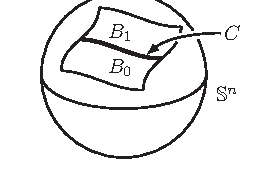
\includegraphics[width=.42\textwidth]{figures/4-9-1.pdf}\\图 4.9.1\end{center}

\textbf{步骤 2：}反设存在上述非零 $\alpha$。根据步骤 1，二等分 $[0,1]$ 后可选其中一个闭区间 $[a_1,b_1]$，长度为 $2^{-1}$，使 $\alpha$ 在 $\widetilde H_i(S^n\setminus D_1)$ 中的像非零，其中 $D_1=h(I^{k-1}\times[a_1,b_1])$。

\sourcepage{237}
再次把该区间二等分，选取使像非零的一半。继续便得到套叠闭区间
\[
[a_1,b_1]\supset[a_2,b_2]\supset\cdots,\qquad b_m-a_m=2^{-m},
\]
及 $D_m=h(I^{k-1}\times[a_m,b_m])$，使 $\alpha$ 在每个 $\widetilde H_i(S^n\setminus D_m)$ 中的像都非零。\translatornote{原书第二次二等分所写的一个端点 $b_2$ 应为 $b_1$；此处统一按递归区间表达。}

设 $\bigcap_m[a_m,b_m]=\{e\}$，则 $E=h(I^{k-1}\times\{e\})=\bigcap_mD_m$ 是 $(k-1)$ 维胞腔。归纳假设给出 $\widetilde H_i(S^n\setminus E)=0$。因此 $\alpha$ 的像在此为零。由定理 4.3.5，存在 $S^n\setminus E$ 中的紧子集 $A$，使 $\alpha$ 已在 $\widetilde H_i(A)$ 中变为零。可先把代表 $\alpha$ 的有限链载体包含在这个紧集内。

但是 $S^n\setminus E$ 是递增开集 $S^n\setminus D_m$ 之并，故紧集 $A$ 包含于其中一个。于是 $\alpha$ 在相应同调群中的像为零，与构造矛盾。\hfill$\square$

\entry{定理}{4.9.4}设 $n>k\ge0$，$h:S^k\to S^n$ 为嵌入，则
\[
\widetilde H_i(S^n\setminus h(S^k))=\begin{cases}\Z,&i=n-k-1,\\0,&\text{其他情形}.\end{cases}
\]
\textbf{证明：}固定 $n$，对 $k$ 归纳。若 $k=0$，像为两点 $p,q$，其补空间同胚于 $\R^n\setminus\{0\}$，而后者同伦等价于 $S^{n-1}$，故结论成立。

设结论对 $k-1$ 成立。取开集 $X_1=S^n\setminus h(E^k_+)$、$X_2=S^n\setminus h(E^k_-)$。令
\[
X=X_1\cup X_2=S^n\setminus h(S^{k-1}),\qquad A=X_1\cap X_2=S^n\setminus h(S^k).
\]
Mayer--Vietoris 序列给出
\[
\begin{split}
\widetilde H_{i+1}(X_1)\oplus\widetilde H_{i+1}(X_2)\longrightarrow
\widetilde H_{i+1}(X)\longrightarrow\widetilde H_i(A)\\
\longrightarrow\widetilde H_i(X_1)\oplus\widetilde H_i(X_2).
\end{split}
\]
\sourcepage{238}
\begin{center}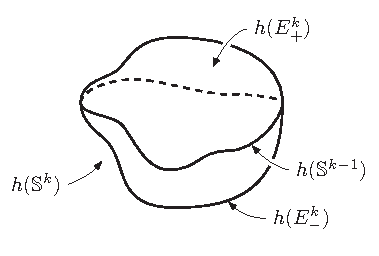
\includegraphics[width=.55\textwidth]{figures/4-9-2.pdf}\\图 4.9.2\end{center}
两个半球的像都是胞腔，所以上一定理说明 $X_1,X_2$ 无环。于是中间映射为同构，亦即
\[
\widetilde H_{i+1}(S^n\setminus h(S^{k-1}))\cong\widetilde H_i(S^n\setminus h(S^k)).
\]
由归纳假设，左端只在 $i+1=n-(k-1)-1$ 时为无限循环群，其余为零，即得结论。\hfill$\square$

\entry{定理}{4.9.5（广义 Jordan 曲线定理）}设 $n>0$，$C\subset S^n$ 同胚于 $S^{n-1}$。则 $S^n\setminus C$ 恰有两个连通分支，$C$ 是二者共同的拓扑边界。

\textbf{证明：}对上一定理取 $k=n-1$，得 $\widetilde H_0(S^n\setminus C)\cong\Z$，故补空间恰有两个道路分支，也就是连通分支 $W_1,W_2$。它们在 $S^n$ 中开，故边界分别为 $\overline W_i\setminus W_i$。只需证明 $\overline W_1\setminus W_1=C$。

由于 $W_2$ 开，它的点不可能是 $W_1$ 的极限点，所以 $\overline W_1\subset S^n\setminus W_2=W_1\cup C$，从而 $\overline W_1\setminus W_1\subset C$。\translatornote{原书此处将 $W_1\cup C$ 误印为 $W_1\cap C$。}

反过来，给定 $x\in C$ 及其邻域 $U$，只需证明它与闭集 $\overline W_1\setminus W_1$ 相交。将 $C$ 分成两个 $(n-1)$ 维胞腔 $C_1,C_2$，使 $C_1$ 足够小而包含于 $U$。图 4.9.3 表示 $n=2$ 的情形。

因为 $C_2$ 不分离 $S^n$，可在 $S^n\setminus C_2$ 中取道路 $\alpha$，连接 $p\in W_1$ 与 $q\in W_2$。该道路必经过 $\overline W_1\setminus W_1$：否则它包含于两个不交开集 $W_1$ 和 $S^n\setminus\overline W_1$ 之并，并同时与两者相交，违背道路像的连通性。

\sourcepage{239}
\begin{center}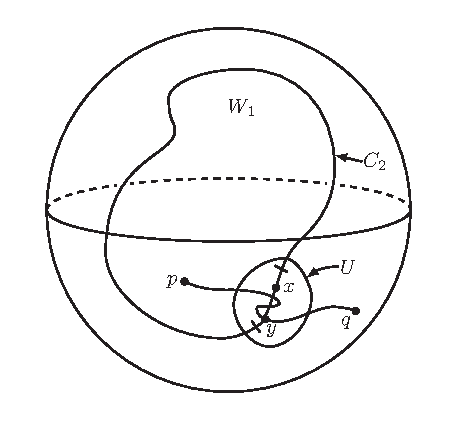
\includegraphics[width=.68\textwidth]{figures/4-9-3.pdf}\\图 4.9.3\end{center}
取道路上的边界点 $y$，则 $y\in C$，且 $y\notin C_2$，故 $y\in C_1\subset U$。因此每个 $U$ 都与该闭边界相交，即得另一包含关系。\hfill$\square$

$S^n$ 的赤道是 $S^{n-1}$ 的同胚像，其补空间两个分支都是开球，闭包都是 $n$ 维胞腔。于是可能猜想，上一定理中的 $\overline W_1,\overline W_2$ 总是 $n$ 维胞腔。$n=2$ 时确实如此，称为 \textbf{Schoenflies 定理}，证明见 [New51]。但 $n>2$ 时需要附加条件。$n\ge3$ 时的广义 Schoenflies 定理由 M. Brown 和 B. Mazur 独立证明，相关论文为 [Maz59]、[Maz61]、[Bro60]、[Mor60]。

三维及更高维中的困难由 J. W. Alexander 于 1924 年在 [Ale24] 中揭示。他构造了后来称为 \textbf{Alexander 角球}（Alexander horned sphere）的曲面。先从环面删去一段，如图 4.9.4 上部，再用圆盘补上两个洞，得到同胚于球面的曲面。接着取两个较小的不完整环面，通过从圆盘小孔伸出的管道，将它们分别接到两张圆盘上。无限重复这一过程。图的下部取自 Alexander 原文，原标记已遮去以免杂乱。

\sourcepage{240}
\begin{center}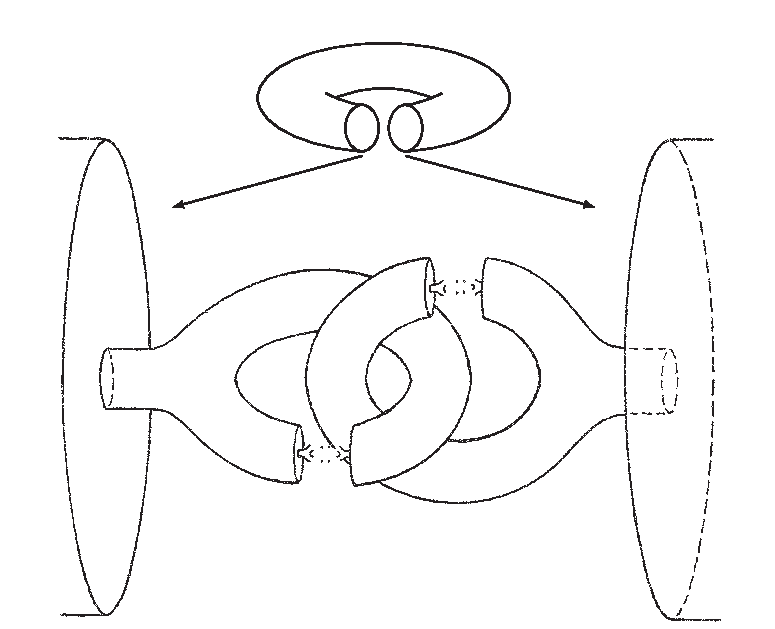
\includegraphics[width=.96\textwidth]{figures/4-9-4.pdf}\\图 4.9.4：Alexander 角球\end{center}
最终曲面同胚于二维球面，但在空间中的嵌入方式与普通圆球面很不相同。若让一条闭曲线穿过其中某个不完整环面看似存在的洞，就不能在始终不碰到角球的条件下把它缩为一点。

经典 Jordan 曲线定理通常对嵌入 $\R^n$ 的球面陈述，而不是嵌入 $S^n$ 的球面。\footnote{长期以来常有人说 Jordan 未成功证明以其命名的定理。其法文原始论述见 [Jor14] 第 587--594 页，读者可自行研究并判断论证的有效性。}下面证明这一版本。

\entry{推论}{4.9.6}设 $n\ge2$，$C\subset\R^n$ 同胚于 $S^{n-1}$。则 $\R^n\setminus C$ 恰有两个连通分支，$C$ 为二者共同的拓扑边界。

\sourcepage{241}
\textbf{证明：步骤 1。}先证明 $S^n$ 的连通开集 $U$ 中，没有一点能够分离 $U$。反设 $U\setminus\{p\}$ 不连通。取足够小的开球 $B(p,\varepsilon)\subset U$，其穿孔部分同胚于 $\R^n\setminus\{0\}$，因 $n\ge2$ 而连通，故包含于某一分支 $D$。令 $E$ 为其余分支之并，则 $E$ 非空，且 $p$ 不是 $E$ 的极限点。因此 $D\cup\{p\}$ 与 $E$ 是不交、非空、开且并为 $U$ 的集合，与连通性矛盾。

\textbf{步骤 2。}将 $\R^n$ 视为 $S^n\setminus\{p\}$，其中 $p$ 为北极。由上一定理，$S^n\setminus C$ 有两个分支 $W_1,W_2$，可设 $p\in W_1$。由步骤 1，$W_1\setminus\{p\}$ 连通，所以它与 $W_2$ 恰为 $(S^n\setminus\{p\})\setminus C$ 的两个分支。它们在该空间中的边界均为 $C$。\hfill$\square$

\entry{定理}{4.9.7（区域不变性）}设 $U\subset\R^n$ 开，$f:U\to\R^n$ 连续且单射。则 $f(U)$ 在 $\R^n$ 中开，且 $f:U\to f(U)$ 是同胚。

\textbf{证明：}可以用 $S^n$ 代替 $\R^n$。

\textbf{步骤 1。}给定 $y\in f(U)$，令 $f(x)=y$。取足够小的开球 $B(x,\varepsilon)$，使闭包 $\overline{B(x,\varepsilon)}\subset U$。记球面 $S(x,\varepsilon)=\overline{B(x,\varepsilon)}\setminus B(x,\varepsilon)$，见图 4.9.5。连续单射在这个紧球上的限制是嵌入，因此 $f(S(x,\varepsilon))$ 同胚于 $S^{n-1}$。由定理 4.9.5，其补空间有两个开分支 $W_1,W_2$。

集合 $f(B(x,\varepsilon))$ 连通且与该球面不交，可设它包含于 $W_1$。它必须等于 $W_1$；否则
\[
S^n\setminus\bigl[f(B(x,\varepsilon))\cup f(S(x,\varepsilon))\bigr]
=S^n\setminus f(\overline{B(x,\varepsilon)})
\]
同时含有整个 $W_2$ 及 $W_1$ 的一些点，因而不连通。这与定理 4.9.3 矛盾，因为 $f(\overline{B(x,\varepsilon)})$ 是一个胞腔。因此 $f(U)$ 包含 $y$ 的开邻域 $W_1$，从而为开集。

\textbf{步骤 2。}将步骤 1 用于 $U$ 的每个开子集，说明 $f$ 是开映射，因此是到其像的同胚。\hfill$\square$

\sourcepage{242}
\begin{center}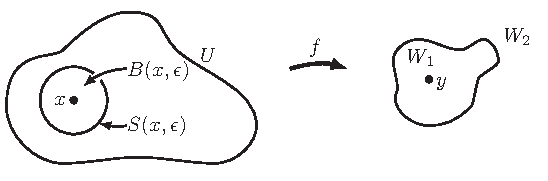
\includegraphics[width=.8\textwidth]{figures/4-9-5.pdf}\\图 4.9.5\end{center}
若额外假设 $f$ 连续可微且 Jacobian 非奇异，区域不变性可由分析中的反函数定理较容易地推出。它的深刻之处是只需要连续性和单射性。同样，当嵌入 $S^{n-1}\to\R^n$ 是某个三角剖分上的单纯映射，或是 Jacobian 具有最大秩的可微映射时，Jordan 曲线定理也较容易证明；真正的困难在于只假设连续且单射。

\subsection*{习题}
\begin{enumerate}
\item 设 $M$ 是第 4.8 节定义的带边界 $m$ 维流形。利用区域不变性证明：
\begin{enumerate}[label=(\alph*)]
\item 若一点在一个坐标片下映到 $\R^{m-1}\times\{0\}$，则在每个坐标片下都如此。
\item 若 $U\subset\R^m$、$V\subset\R^n$ 为非空开集且彼此同胚，则 $m=n$。
\item 数 $m$ 由 $M$ 唯一确定。
\end{enumerate}
\item \begin{enumerate}[label=(\alph*)]
\item 设 $Y$ 为拓扑学家的正弦曲线（定义 4.2.11）。证明：若 $h:Y\to S^n$ 为嵌入，则 $S^n\setminus h(Y)$ 无环。
\item 设 $X$ 为闭合的拓扑学家正弦曲线（定义 4.6.5）。证明：若 $h:X\to S^n$ 为嵌入，则 $\widetilde H_i(S^n\setminus h(X))$ 在 $i=n-2$ 时为无限循环群，其余为零。
\item 设 $X$ 同 (b)，若 $h:X\to S^2$ 为嵌入，证明其补空间恰有两个分支，且 $h(X)$ 为共同拓扑边界。
\end{enumerate}
\sourcepage{243}
\begin{center}
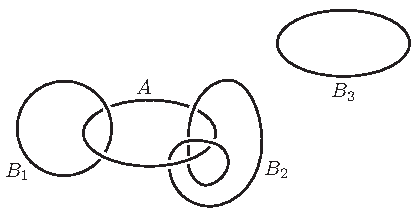
\includegraphics[width=.65\textwidth]{figures/4-9-6.pdf}\\图 4.9.6\par\medskip
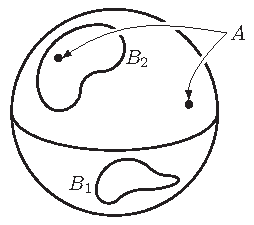
\includegraphics[width=.4\textwidth]{figures/4-9-7.pdf}\\图 4.9.7
\end{center}
\item \begin{enumerate}[label=(\alph*)]
\item 将 $S^3$ 视为添加了无穷远点的 $\R^3$。设 $A,B_1,B_2,B_3$ 为图 4.9.6 中的简单闭曲线。包含映射诱导的 $H_1(B_i)\to H_1(S^3\setminus A)$ 是无限循环群间的同态，因而为乘以一个除符号外确定的整数 $d_i$。它度量 $B_i$ 与 $A$ 环绕的次数。分别求这些整数；再求 $H_1(A)\to H_1(S^3\setminus B_i)$ 的相应整数。你能提出什么猜想？
\item 设 $A$ 为 $S^2$ 的两个点，$B_1,B_2$ 为图 4.9.7 中的简单闭曲线。求包含映射诱导的同态
\[
\widetilde H_0(A)\to\widetilde H_0(S^2\setminus B_i),\qquad H_1(B_i)\to H_1(S^2\setminus A),
\]
并提出猜想。
\item 对 $S^{p+q+1}$ 中不相交的 $S^p,S^q$ 的嵌入提出一个猜想。证明 Alexander 对偶定理后将再次讨论它，见第 8.12 节习题。
\end{enumerate}
\item 在三维中，对边界曲面作适当光滑性假设，可以得到 Jordan 曲线定理的一种加强形式。这是 Mazur 与 Brown 的著名结果。讨论可能的表述。
\end{enumerate}
